\documentclass[aps,onecolumn, notitlepage, longbibliography]{revtex4-1}
%\linespread{2}

\usepackage{graphicx}% Include figure files
\usepackage{dcolumn}
\usepackage{bm}% bold math
\usepackage[colorlinks=true,bookmarks=false,citecolor=blue,linkcolor=blue,hyperfootnotes=true,urlcolor=blue]{hyperref}
\usepackage{color}
\usepackage{comment}

\DeclareRobustCommand{\element}[1]{\@element#1\@nil}
\def\@element#1#2\@nil{%
  #1%
  \if\relax#2\relax\else\MakeLowercase{#2}\fi}
\pdfstringdefDisableCommands{\let\element\@firstofone}
\makeatother

\begin{document}

\title{Notes for MULTIPLETY: A Python wrapper for Fortan-based multiplet calculations}


%\author{G. Fabbris}
%\author{M. P. M. Dean}
%\email{mdean@bnl.gov}


% user macros
\def\mathbi#1{\ensuremath{\textbf{\em #1}}}
\def\Q{\ensuremath{\mathbi{Q}}}
\def\LNO{LaNiO$_3$}
\newcommand{\angstrom}{\mbox{\normalfont\AA}}
\date{\today}

% insert suggested PACS numbers in braces on next line
\pacs{74.70.Xa,75.25.-j,71.70.Ej}
% insert suggested keywords - APS authors don't need to do this
%\keywords{}
%
%\maketitle must follow title, authors, abstract, \pacs, and \keywords
\maketitle

MULTIPLETY provides a python wrapper for performing simple atomic calculations of RIXS spectra based Cowan's and the Racer codes. The approach is primairly for internal use at Brookhaven National Laboratory and largely mirrors what was implemented by Stavitski and de Groot \cite{Stavitski2010}, but with the flexibility to choose the x-ray polarization. 

\section{Theory primer}

The multiplet method starts by computing atomic wavefunctions via the Hartree-Fock method using Cowan's codes \cite{CowmanBook}. Crystal fields are then introduced by mixing the atomic functions to generate the appropriate symmetry orbitals using Theo Thole's Racer code. $L$-edge RIXS involves two dipolar transitions via an intermediate state with a $p$ core hole for example $2p^63d^8 \rightarrow 2p^53d^9  2p^63d^8*$ where $*$ denotes an orbital $dd$-transition \cite{Ament2011}. The matrix elements for these transitions are calculated for dipole operators appropriate for the incident and final x-ray polarization and RIXS is then computed using the Kramers-Heisenberg equation. The effects of electron-electron interactions are incorporated using the Slater-Condon parameters. $F_{dd}$ and $F_{pd}$ set the percentage reductions in the Coulomb repulsion between two $d$ electrons and $p$-$d$ electrons respectively \cite{deGrootBook, deGroot2005}. $G_{pd}$ is the percentage reduction in the Coulomb exchange. 

\section{Practicalities}

\subsection{Polarization}

A typical experimental RIXS geometry is shown in Fig.~\ref{geom}. Vertically ($\sigma$) or horizontally ($\pi$) polarized x-rays are incident at $\theta_i$ on the sample. The incident x-ray electric field ($\vec{e}$) is always parallel to $b$ for $\sigma$ polarization. On the other hand, $\pi$ incident x-ray polarization probes a mixture of $\vec{e} \parallel c$ and $\vec{e}\parallel a$ contributions.  Such a geometry is handled via \texttt{generate\_polarization}($\theta_i$, $2\theta$). Other geometries can be handled by constructing and passing \texttt{absorption\_pol} and \texttt{emission\_pol} to 
\texttt{calculate\_rixs} by hand. The codes uses a basis with two helical and one linear component, which are defined with respect to the high symmetry direction of the atomic site, which we will refer to as the $c$-axis. Right and left circularly polarized light are represented as
\begin{equation}
(1, 0, 0)
\end{equation}
and
\begin{equation}
(0, 0, 1).
\end{equation}
Linear light along the $a$, $b$ and $c$ axes is then represented as
\begin{equation}
\frac{1}{\sqrt{2}}(1, 0, 1), 
\end{equation}
\begin{equation}
\frac{i}{\sqrt{2}}(1, 0, -1),
\end{equation}
and
\begin{equation}
(0, 1, 0).
\end{equation}

For the case in which only one polarization component is measured, one should set this direction as \texttt{emission\_pol}. If the measurement is performed without polarization analysis \texttt{emission\_pol} should be set as a equal combination of both polarizations perpedicular to the direction of the light. 

\subsection{Running the code}


\begin{figure}
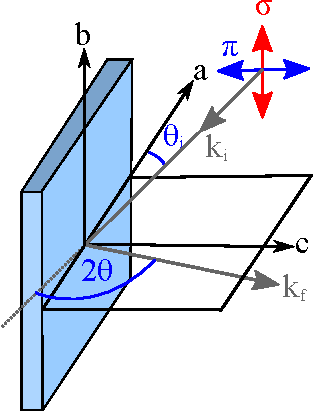
\includegraphics[width=1.7 in]{suppl_geometry.pdf}
\caption{RIXS scattering geometry. Linearly polarized x-rays ($\sigma$ or $\pi$) are incident upon the sample at an angle $\theta _i $. The scattered photons are collected at $2\theta$ and measured as a function of final energy.}
\label{geom}
\end{figure}

The core of the code happens in \texttt{atomic\_calculation.py}, which creates the input files and runs the Fortran executables:
\begin{enumerate}
\item \texttt{rcn} and \texttt{rcn2} which calculate the atomic radial wavefunctions
\item \texttt{rcg} which calculates the atomic energy levels and spectra
\item \texttt{racer}: introduces the crystal field and magnetic exchange. Note that the
states are given using Butler notation (see \href{https://github.com/gfabbris/multiplety/blob/master/multiplety/atomic\_calculation.py}{atomic\_calculation.py}).
\item \texttt{calc\_exc}, which organizes the excitation energies calculated by \texttt{racer}.
\item \texttt{cleanup}, which moves all files to the selected folder.
\end{enumerate}

One RIXS process involves running this twice to compute the absorption (intial to intermedate states) transition and then the emission (intermediate to final state) processes. \texttt{process\_rixs} reads the transition matrices \texttt{abs\_racer\_out.ora} and \texttt{emi\_racer\_out.ora} created in the first step, applies the x-ray polarization and Boltzmann factors and put all the transition into the Kramer-Heisenberg formula to calculate the spectrum. 

\bibliography{refs}

\end{document}
